%%%%%%%%%%%%%%%%%%%%%%%%%%%%%%%%%%%%%%%%%%%%%%%%%%%%%%%%%%%%%%%%%%%%%%
%%%%%%%%%%%%%%%%%%%%%%%%%%%%%%%%%%%%%%%%%%%%%%%%%%%%%%%%%%%%%%%%%%%%%%
%%%%%%%%%%%%%%%%%%%%%%%%%%%%%%%%%%%%%%%%%%%%%%%%%%%%%%%%%%%%%%%%
%   kmake afb_sig2-ps
\documentclass[12pt]{article}


%%%%%%%%%%%%%%%%%%%%%%%%%%%%%%%%%%%%%%%%%%%%%%%%%%%%%%%%%%%%%%%%%
\usepackage{epsfig}

\usepackage{amsmath}
\usepackage{amssymb}
\usepackage{euscript}

\usepackage{fancybox}
\usepackage{xcolor}


%%%%%%%%%%%%%%%%%%%%%%%%%%%%%%%%%%%%%%%%%%%%%%%%%%%%
\input Energy.tex
\input Process.tex
%\def\Energy{MZ-1.8GeV (had.)}
\def\Angle{$\theta^{\bullet}$}


%%%%%%%%%%%%%%%%%%%%%%%%%%%%%%%%%%%%%%%%%%%%%%%%%%%%%%%%%%%%%%%
%  copied from seminar.con
\def\titbox#1{\begin{center}\doublebox{#1}\end{center}}

\newcommand{\KK}{${\cal KK}$}
%--------------------------------------------------------------
\def\Order#1{${\cal O}(#1)$}
\def\Ordpr#1{${\cal O}(#1)_{prag}$}
\def\Oceex#1{${\cal O}(#1)_{_{\rm CEEX}}$}
\def\Oeex#1{${\cal O}(#1)_{_{\rm EEX}}$}
\def\OrderLL#1{${\cal O}(#1)_{\rm LL}$}


%%%%%%%%%%%%%%%%%%%%%%%%%%%%%%%%%%%%%%%%%%%%%%%%%%%%%%%%%%%%%%%
\textwidth  = 16cm % <-- maximum CERN
\textheight = 22cm % <-- maximum CERN
\hoffset    = -1cm
\voffset    = -1cm


%%%%%%%%%%%%%%%%%%%%%%%%%%%%%%%%%%%%%%%%%%%%%%%%%%%%%%%
%%%%%%%%%%%%%%%%%%%%%%%%%%%%%%%%%%%%%%%%%%%%%%%%%%%%%%%
\begin{document}                     %%%%%%%%%%%%%%%%%%


%//////////////////////////////////////////////////////////////////////////////////
%//////////////////////////////////////////////////////////////////////////////////
%//////////////////////////////////////////////////////////////////////////////////
\titbox{{\large\bf\color{red} CEEX $\sigma$ and $A_{\rm FB}$, 
                              energy cut-off study }}


{\bf\large Process \Process, at \Energy.}

\begin{center}
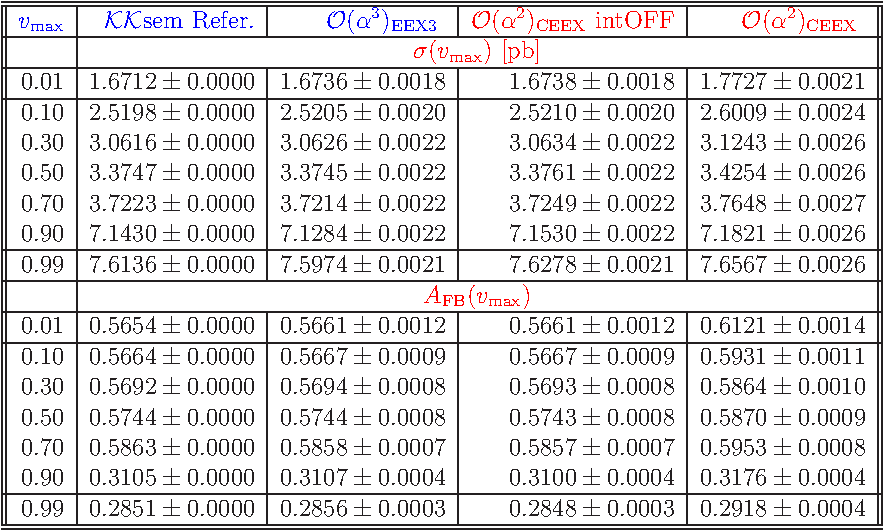
\epsfig{file=afb_int2-tab1.eps,width=160mm}
\end{center}

\large
Energy cut: $v<v_{\max}$, $v=1-M^2_{f\bar{f}}/s$.
Scattering angle for $A_{\rm FB}$ is $\theta=$\Angle.
No cut in \Angle.
E-W corr. in \KK\  according to DIZET 6.x.
EEX3 is \OrderLL{\alpha^3} EEX3 matrix element without ISR$\otimes$FSR interf.
\KK{}sem is semianalytical part of \KK.
{\small (Angle $\theta^{\bullet}$ is from Phys. Rev. {\bf D41}, 1425 (1990).)}
\\
Table III in Phys.Rev. D63 (2001) 113009.\\
Table I in  Phys.Rev. D88 (2013) no.11, 114022.


%-----------------------------------------------------------
\vfill


%//////////////////////////////////////////////////////////////////////////////////
%//////////////////////////////////////////////////////////////////////////////////
%//////////////////////////////////////////////////////////////////////////////////
\newpage
\titbox{{\large\bf\color{magenta} Total cross section $\sigma$, energy cut-off stydy}}

\begin{center}
\epsfig{file=afb_int2-Gsig.eps,width=160mm}
\end{center}

The same as in the table. No cut in \Angle.
Ref. $\sigma_{\rm ref}$ = semianalytical of \KK{}sem.
%-----------------------------------------------------------
\vfill

%//////////////////////////////////////////////////////////////////////////////////
%//////////////////////////////////////////////////////////////////////////////////
%//////////////////////////////////////////////////////////////////////////////////
\newpage
\titbox{{\large\bf\color{magenta} Charge asymmetry $A_{\rm FB}$, energy cut-off study}}

\begin{center}
\epsfig{file=afb_int2-Gafb.eps,width=160mm}
\end{center}

The same as in the table.
No cut in \Angle.
Reference $A_{\rm FB}^{\rm ref}$ =  semianalytical \KK{}sem.

%-----------------------------------------------------------
\vfill


%//////////////////////////////////////////////////////////////////////////////////
%//////////////////////////////////////////////////////////////////////////////////
%//////////////////////////////////////////////////////////////////////////////////
\newpage
\titbox{{\large\bf\color{magenta} 
                      Physical Precision of CEEX ISR }}


%-----------------------------------------------------------
\begin{center}
\epsfig{file=afb_int2-sigHO.eps,width=100mm}
\epsfig{file=afb_int2-afbHO.eps,width=100mm}
\end{center}

The difference between second and first order CEEX results for at \Energy.\\
The energy cut is on $s'/s$, where $s'=m^2_{f\bar{f}}$.

{\color{blue} Scattering angle is $\theta=$\Angle. }
{\small\color{blue} [Angle $\theta^{\bullet}$ is defined in Phys. Rev. {\bf D41}, 1425 (1990)]}

%-----------------------------------------------------------
\vfill




\end{document}

